%========================================================================================================
\section{Tree Statistics Using \citet{SUSSING_HALOFINDER} Selection Criteria}\label{app:performance_comparison}
%========================================================================================================



\begin{table}
\centering
\caption{
	Comparison of simulation and evaluation parameters used in this work and of A14, where the parameters of the latter have been converted using $h = 0.704$.
	$m_m$ is the mass threshold for main haloes, $m_s$ is the mass threshold for sub-haloes.
	\label{tab:parameter-comparison}
}
	\begin{tabular}[c]{l l l}
																	&	This work		&	A14 \\
		\hline
		particle mass	[$10^9 \msol$]	&	$1.55$			& $1.32$						\\
		particles used								& $256^3$			& $270^3$ 					\\
		box size [Mpc/h]							& $62.5$			& $62.5$						\\
		snapshots until $z = 0$				& 62					& 62								\\				
		$m_m$ [$10^{12} \msol$]				&	$1.35$			& $1.12$ - $1.37$		\\
		$m_s$ [$10^{11} \msol$]				&	$4.03$			& $4.26$ - $9.72$		\\
		\hline
	\end{tabular}
\end{table}


\begin{figure}
	\centering
	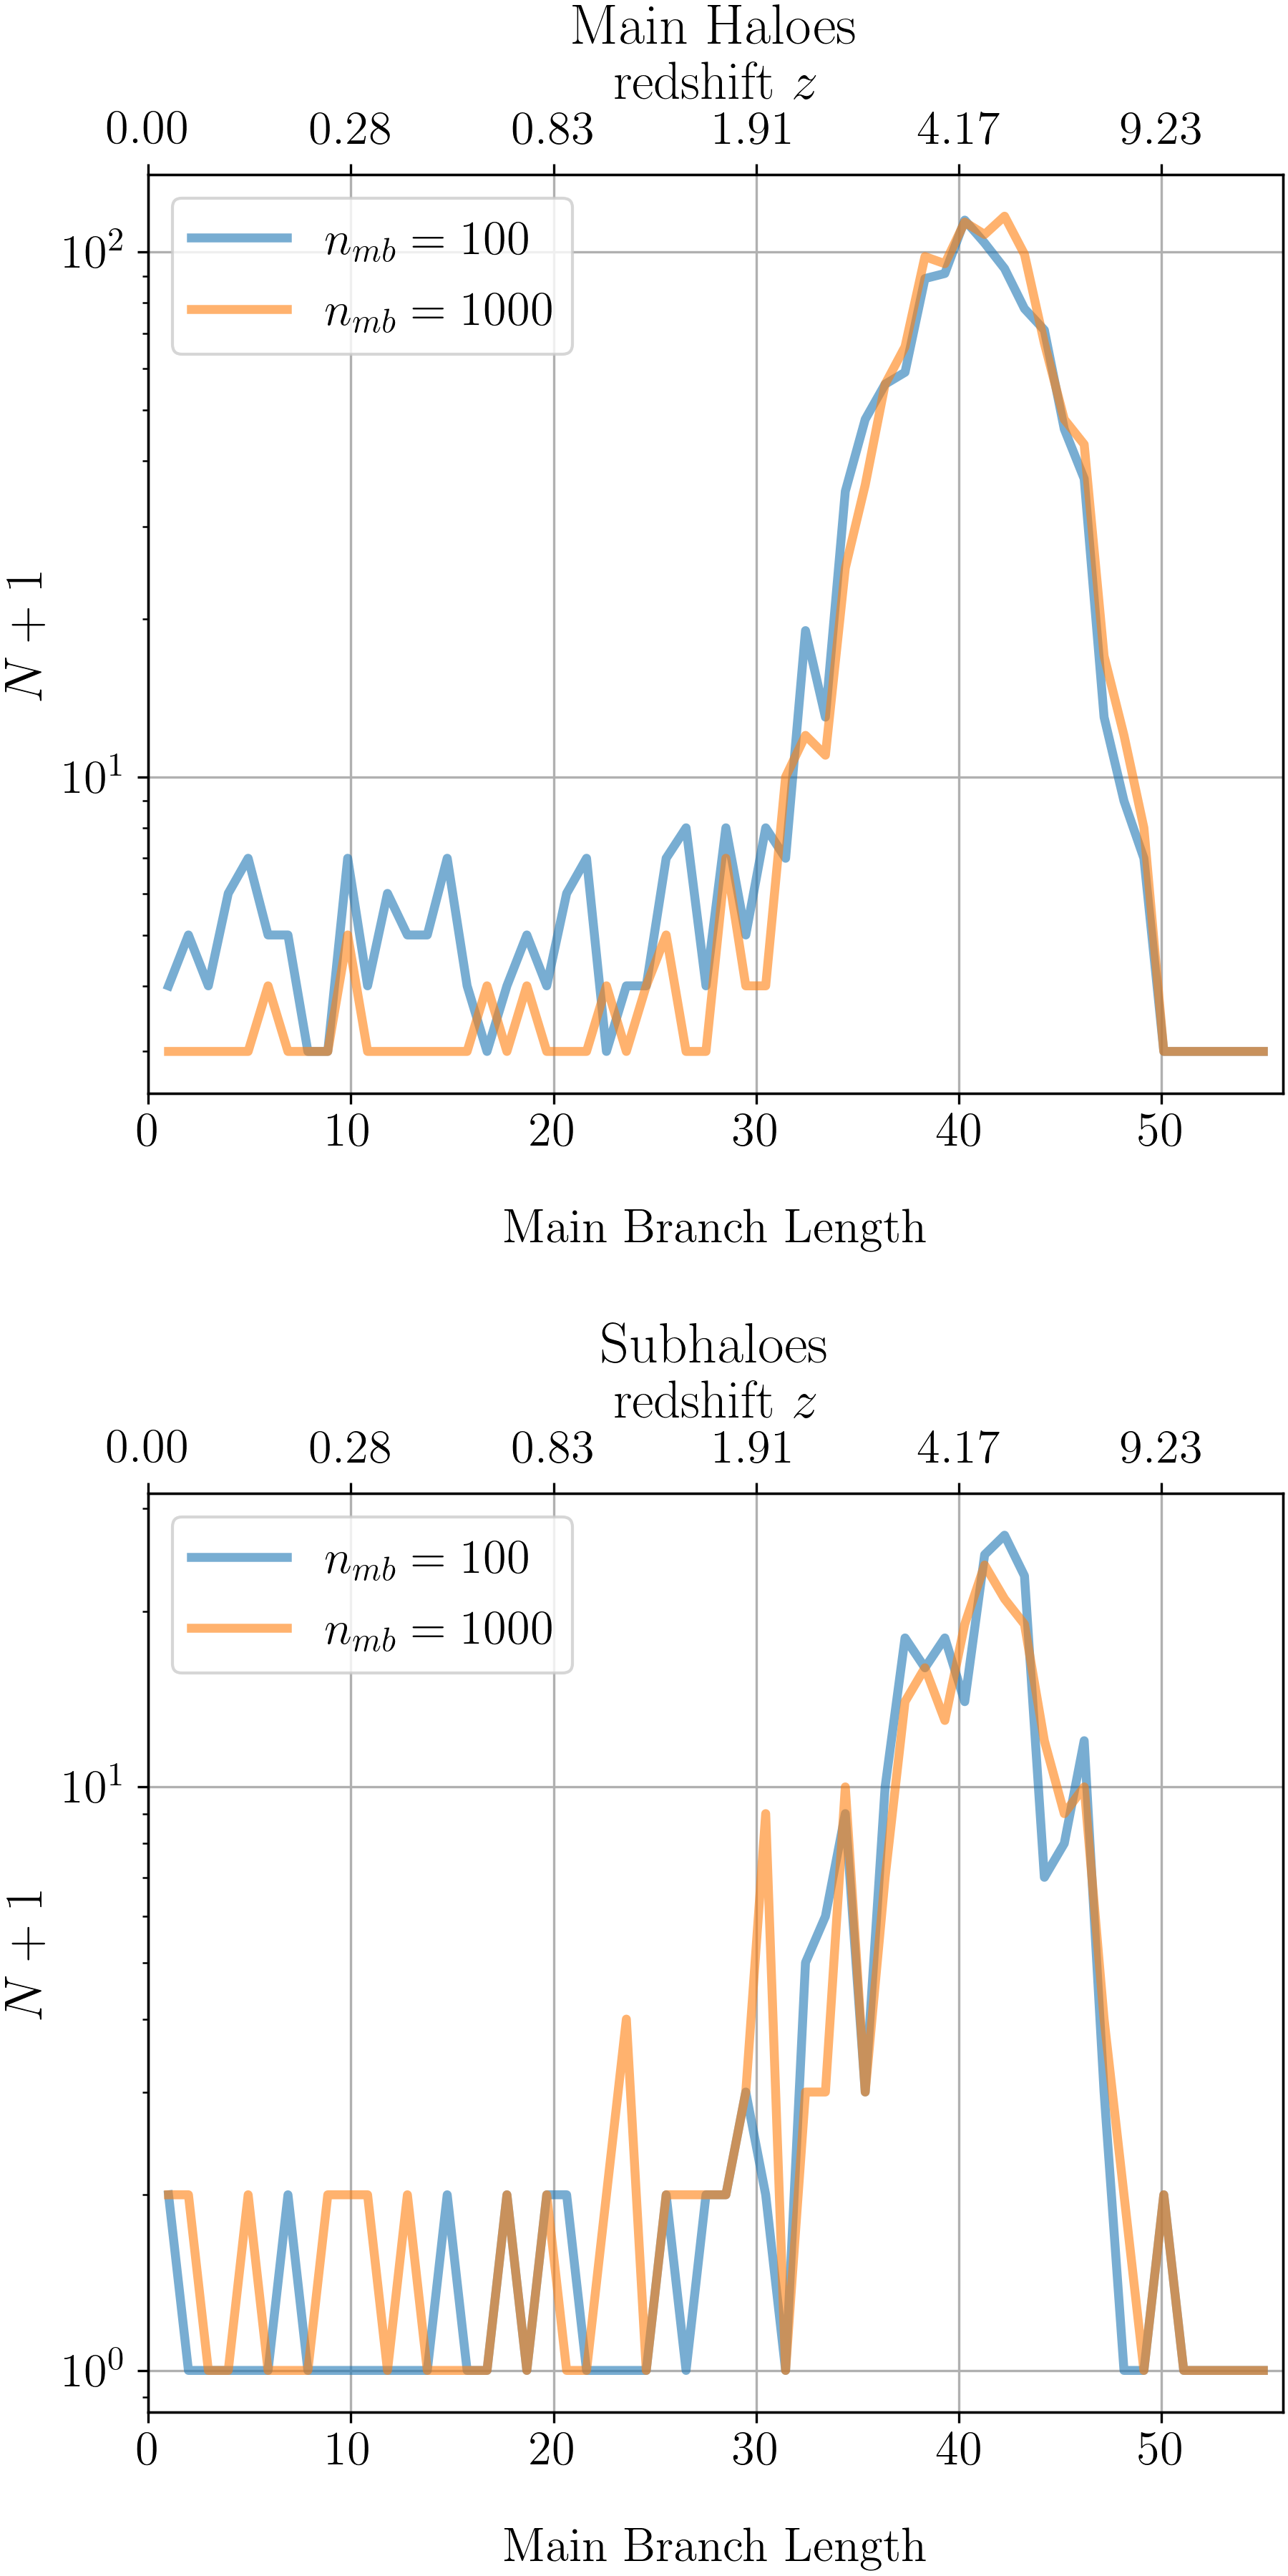
\includegraphics[width=.95\linewidth, 
	keepaspectratio]{images/tree-statistics-sussing-threshold/main-branch-lenghts-all-bins-ntrace.png}%
	\caption{
		Histograms of the length of the main branch. 
		The top plot shows the length of the 1000 most massive haloes at $z = 0$, the bottom plot shows 
		the length of the 200 most massive sub-haloes for $n_{mb} = 100$ and $1000$ tracer particles 
		per clump.
	}%
	\label{fig:sussing-branch-lengths}
\end{figure}


\begin{figure}
	\centering
	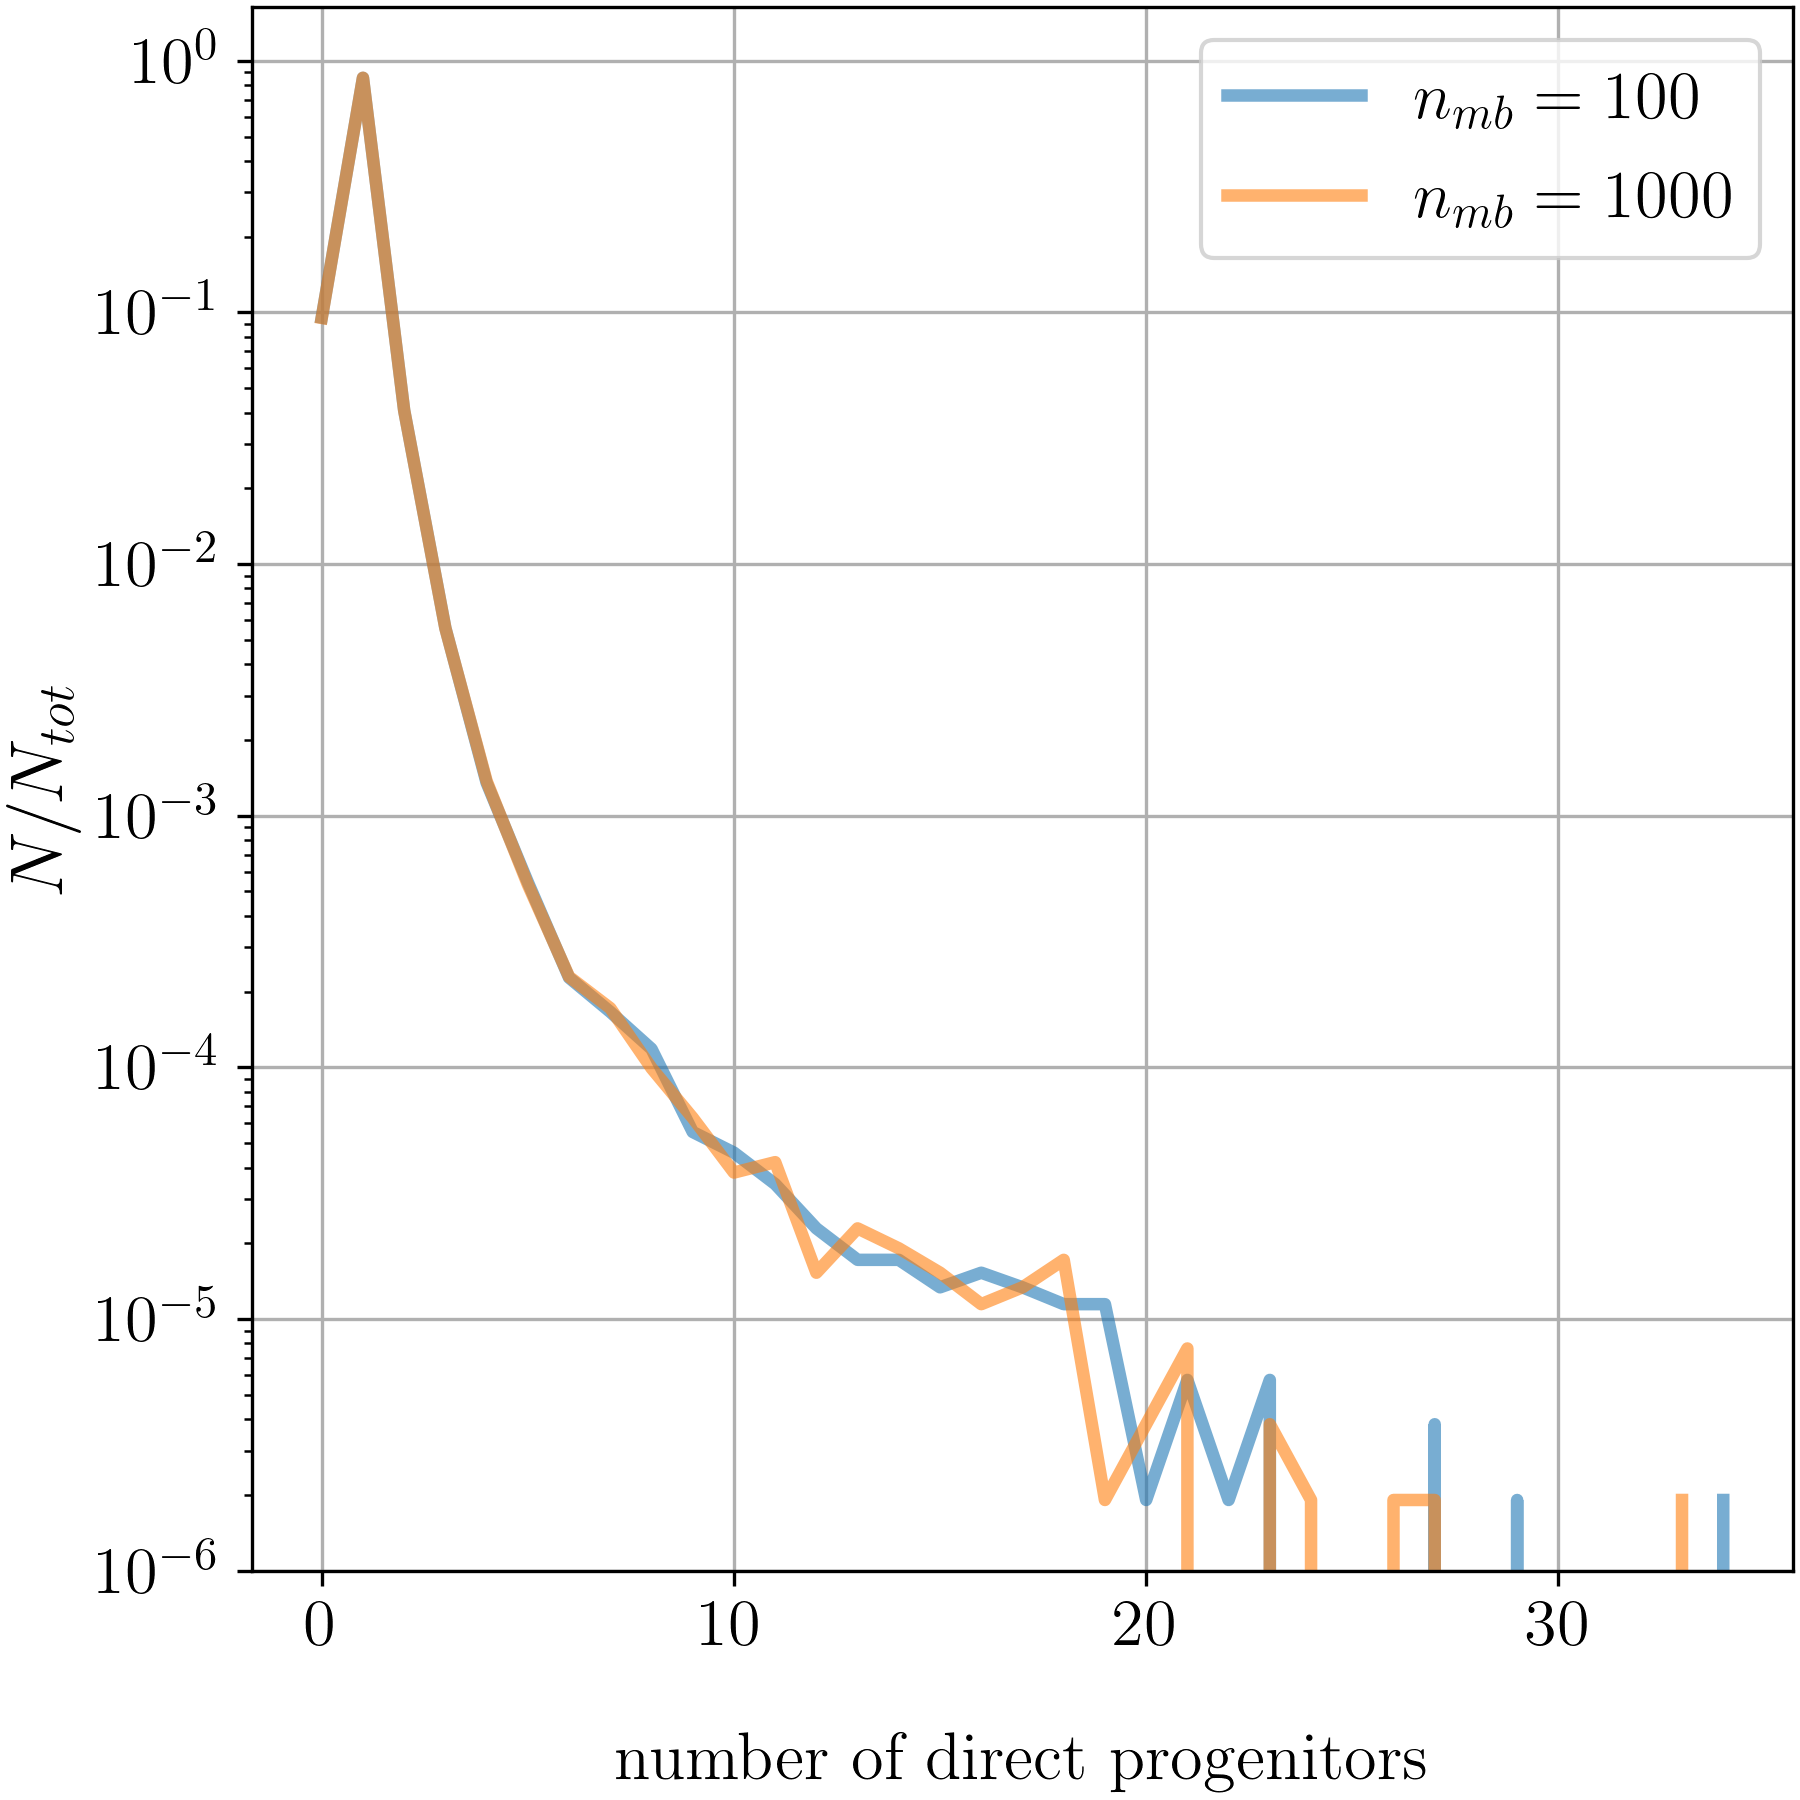
\includegraphics[width=.9\linewidth, keepaspectratio]{images/tree-statistics-sussing-threshold/branching-ratio-ntrace.png}\\%
	\caption{
		Histogram of the number of direct progenitors for all clumps from $z = 0$ to $z = 2$ for $n_{mb} = 100$ and $1000$ tracer particles per clump.
		The histogram is normalized by the total number of events found.
	}%
	\label{fig:sussing-branching-ratio}
\end{figure}


\begin{figure*}
	\centering
	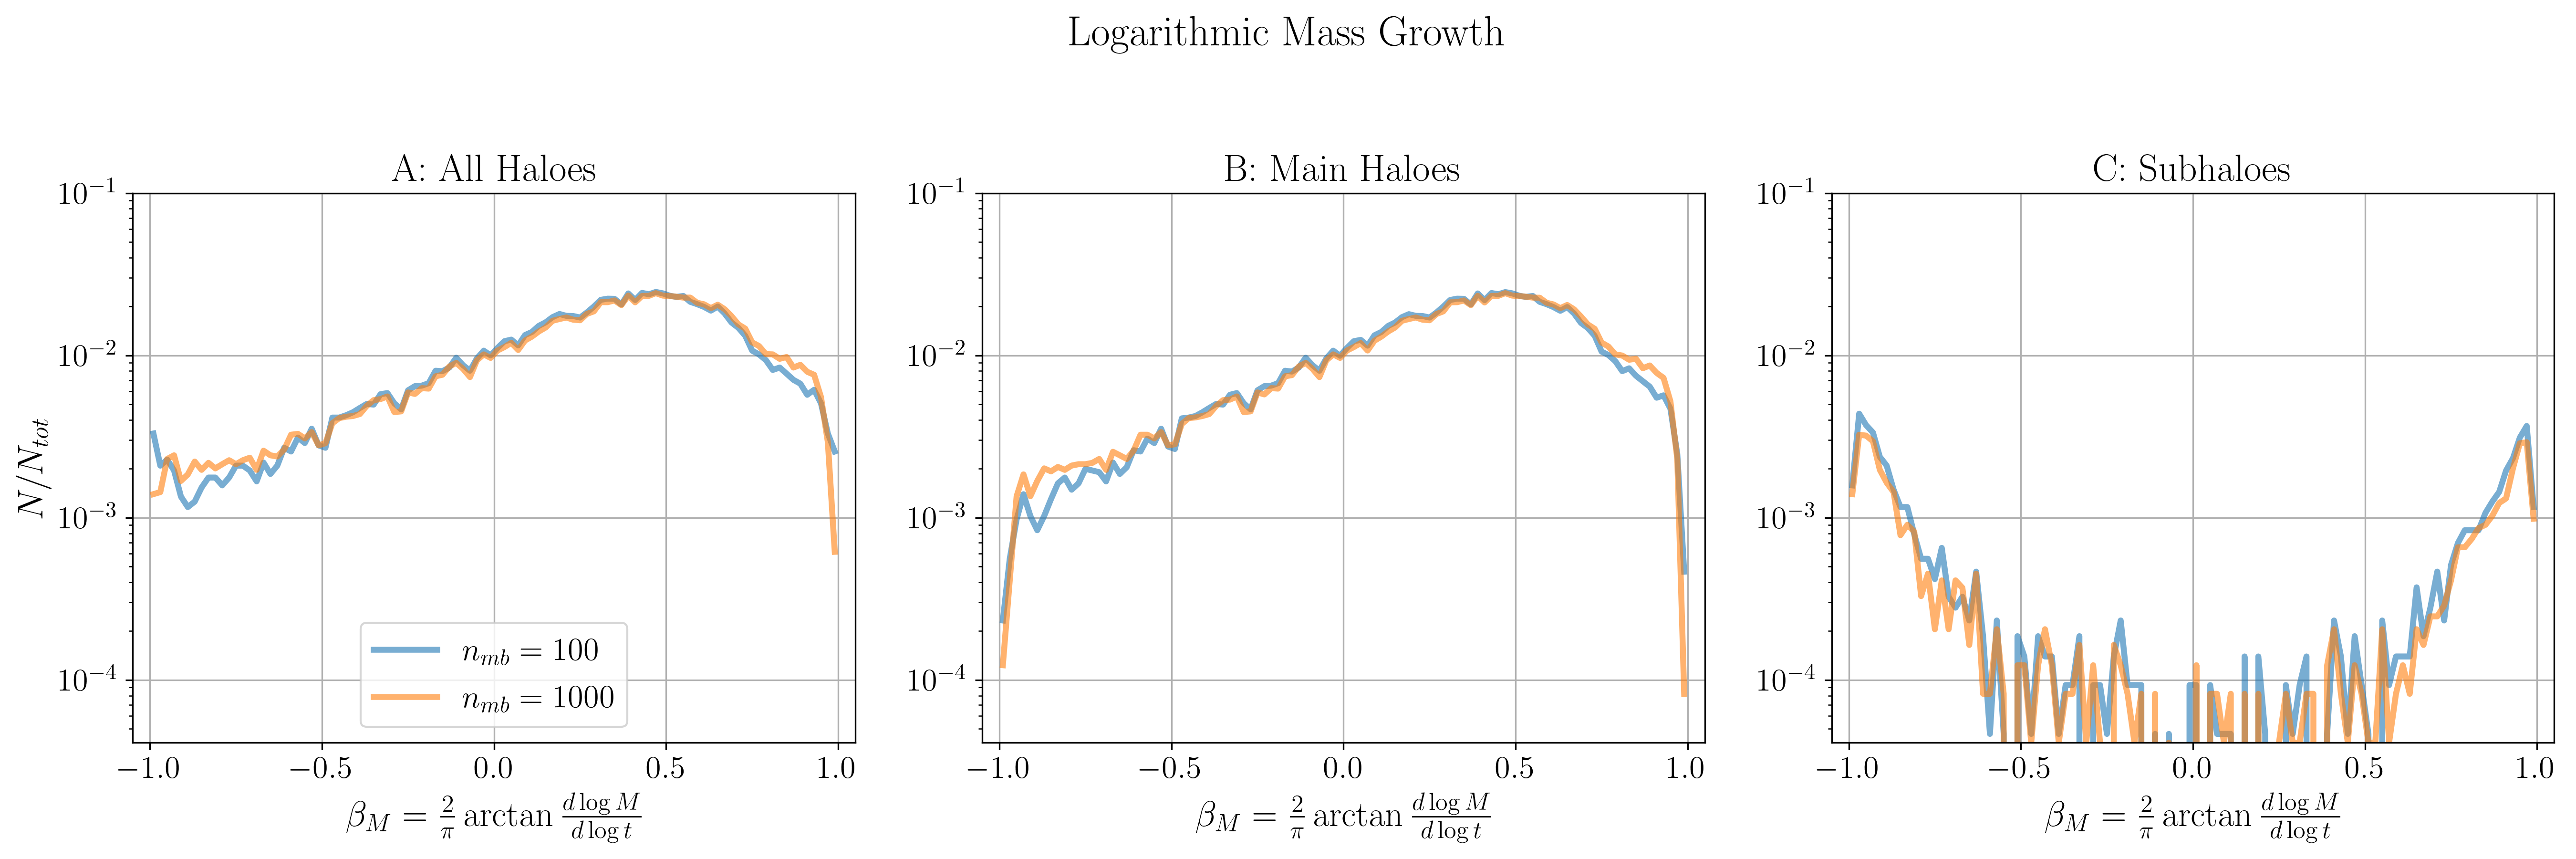
\includegraphics[width=\textwidth, keepaspectratio]{images/tree-statistics-sussing-threshold/mass_growth-ntrace.png}%
	\caption{
		Logarithmic mass growth for haloes and sub-haloes satisfying the mass thresholds.
		Group $A$ contains clumps that are either haloes or sub-haloes in consecutive snapshots $k$ and $k+1$ with masses $m \geq m_{m}$.
		Group $B$ contains clumps that are only haloes in two consecutive snapshots with mass above $m_{m}$, group $C$ contains only clumps that were sub-haloes in two consecutive snapshots with mass greater than $m_{s}$.
		The histogram is normalized by the total number of events found for group $A$.
	}%
	\label{fig:sussing-mass-growth}
\end{figure*}

\begin{figure*}
	\centering
	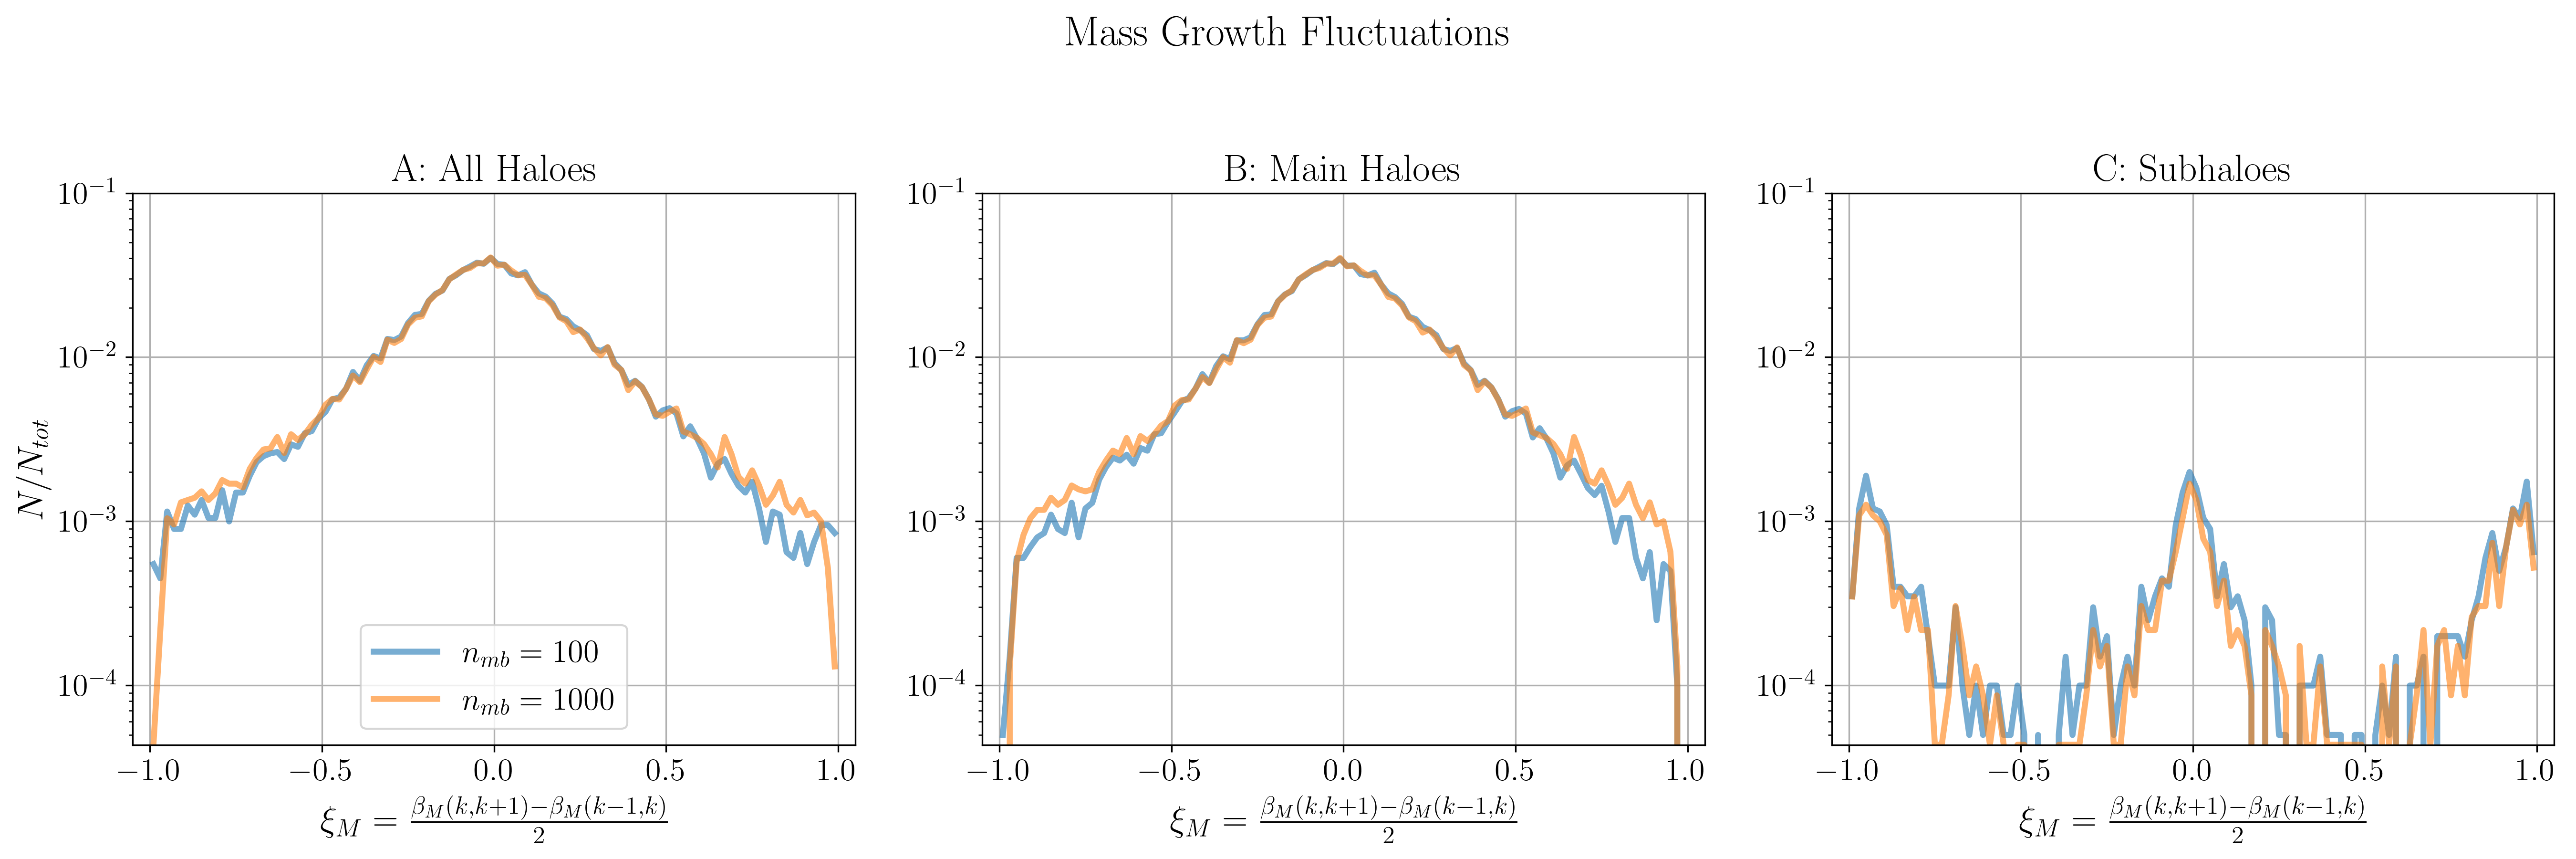
\includegraphics[width=\textwidth, keepaspectratio]{images/tree-statistics-sussing-threshold/mass_fluctuations-ntrace.png}\\%
	\caption{
		Histogram of mass growth fluctuations for haloes and sub-haloes satisfying the mass thresholds.
		Group $A$ contains clumps that are either haloes or sub-haloes in three consecutive snapshots with masses $m \geq m_{m}$.
		Group $B$ contains clumps that are only haloes in three consecutive snapshots with mass above $m_{m}$, group $C$ contains only clumps that were sub-haloes in three consecutive snapshots with mass greater than $m_{s}$.
		The histogram is normalized by the total number of events found for group $A$.
	}%
	\label{fig:sussing-mass-fluct}
\end{figure*}




In this section, the merger tree statistics introduced in Section \ref{chap:tests} when following the selection criteria that are used in \citet{SUSSING_HALOFINDER} (A14 from here on) are presented.
Ideally, \texttt{ACACIA} should be tested on the same datasets and halo catalogues used in the Comparison Project to enable a direct comparison to the performance of other merger tree codes. 
However, since \texttt{ACACIA} was designed to work on the fly, using it as a post-processing utility would defeat its purpose.
Furthermore, \texttt{ACACIA} is not necessarily compatible with other definitions of haloes and sub-haloes.
But most importantly, we also want to demonstrate that the halo finder \phew\ can be used to produce reliable merger trees. 
So instead, the tests are performed on our own datasets and halo catalogues, which are described in section \ref{chap:testing_methods}.
A comparison of the used parameters of our simulations and the ones used in A14 is given in Table \ref{tab:parameter-comparison}.
In the following, the results for $n_{mb} = 100$ and $n_{mb} = 1000$ are shown.
Like before, when the influence of the number of tracer particles was investigated, the \sad\ parameter and the \exc\ mass definition were used.


The difference to the results presented in Section \ref{chap:tests} is that the mass thresholds are set such that only the 1000 most massive main haloes and only the 200 most massive sub-haloes at $z = 0$ are included.
This gives effective mass threshold $m_{m} = 1.35 \times 10^{12} \msol$ and $m_{s} = 4.0 \times 
10^{11}\msol$, which are on one hand comparable to the mass thresholds applied in A14 (Table 
\ref{tab:parameter-comparison}), but already show differences in the resulting halo catalogue.
\phew\ finds a mass threshold for main haloes that is close to the upper limit found in A13, 
but a lower mass threshold for sub-haloes.
This is consistent with the fact that the \sad\ parameter was used:
Unbound particles are passed on to substructure that is higher up in the hierarchy, and the unbinding is repeated until the top level, which are the main haloes, is reached.
The more strict unbinding criterion tends to assign more particles to the main haloes and remove them from sub-haloes, which is reflected in the mass thresholds.
Indeed, using the \nosad\ parameter instead leads to $m_m = 1.27 \times 10^{12}\msol$ and $m_s = 
1.92 \times 10^{12}\msol$.



The length of the main branches for haloes and sub-haloes individually are shown in Figure 
\ref{fig:sussing-branch-lengths}. Compared to Figure 3 of A14, we note the following similarities 
and differences:
%
\begin{enumerate}
	\item \texttt{ACACIA} finds some main haloes with short (< 10) main branches.
		In A14, his only happens for the \texttt{JMerge} and \texttt{TreeMaker} tree builders
		regardless	of the halo finder employed, and the \texttt{MergerTree}, \texttt{SubLink}, 
		and \texttt{VELOCIraptor} tree makers for \texttt{AHF} and \texttt{Subfind} halo finders.
%	
	\item Like in nearly all cases in A14, the distribution of main branch lengths for
		main haloes peaks at high numbers and the bulk of the distribution is about 20 snapshots
		wide. The peak of the main branch length distribution of \texttt{ACACIA} is at 40,
		while in most cases in A14, it's around 45 with the exception of the \texttt{AHF}
		halo finder. This indicates that \texttt{ACACIA} and \phew\ result in on average 
		somewhat smaller main branch lengths than other codes. However, we also find the 
		maximal main branch length of 50, while nearly all combinations of
		halo finders and tree makers in A14 find higher values. Both these differences can be 
		explained by the slightly lower resolution that we used in our simulations, where we 
		found no identifiable clumps before snapshot 11, which corresponds to a maximal main 
		branch length of 51. 
%
	\item The main branch lengths for sub-haloes also follow the trends noted above. Additionally,
		the distribution is flat for main branch lengths smaller than 30, which is not the case
		for \texttt{Rockstar} and \texttt{AHF} sub-haloes in A14 for nearly all tree builders. Instead,
		their main branch lengths peak again around unity.
\end{enumerate}
%
In summary, regarding the main branch lengths of main haloes, \phew\ and \texttt{ACACIA} perform
comparably to \texttt{Subfind} and \texttt{Rockstar} halo finders and \texttt{MergerTree}, 
\texttt{TreeMaker}, and \texttt{VELOCIraptor} tree builders. Concerning sub-haloes, the results are
most closely to \texttt{Subfind} sub-haloes and the same tree builders as for the main haloes. This 
is not surprising, because \texttt{Subfind} employs a similar definition of substructure being 
arbitrarily shaped self-bound structure that is truncated at the isodensity contour that is 
defined by the density saddle point between the sub-halo and the main halo. 

In Figure \ref{fig:sussing-branching-ratio} the number of direct progenitors for all clumps between 
$z = 0$ and $z = 2$ are shown. Comparing to Figure 5 of A14, \texttt{ACACIA} gives very comparable 
results: $\sim 10^{-1}$ haloes have no direct progenitor, almost all have one, and the distribution 
follows an exponential decay with the maximal number of direct progenitors lying around 20-25, save 
for a very few outliers. Many tree makers and halo finders in A14 exhibit the same kind of 
behaviour, particularly so for the \texttt{AHF}, \texttt{Subfind}, and \texttt{Rockstar all} halo 
finders in Figure 5 of A14.


For the logarithmic mass growth (Figure \ref{fig:sussing-mass-growth}) and the mass growth fluctuations (Figure \ref{fig:sussing-mass-fluct}), the statistics are separated into three groups.
Group $A$ contains clumps that are either haloes or sub-haloes in \emph{consecutive} snapshots $k$ 
and $k+1$ with masses greater than the mass threshold $m_m$ in both snapshots. Group $B$ contains 
clumps that are exclusively main haloes in two consecutive snapshots with mass above $m_{m}$, group 
$C$ contains only clumps that were sub-haloes in two consecutive snapshots with mass greater than 
$m_{s}$. We follow clumps of the $z = 0$ snapshot along the main branch only.

The logarithmic mass growth resulting from \texttt{ACACIA} follows the general trend that the tree 
makers in A14 exhibit too. The growth for groups $A$ and $B$ increases steadily and peaks around 
$\beta_M \sim 0.5$, where the peak is $\sim2 \times 10^{-2}$. For $n_{mb} = 100$, the extreme mass 
loss  with $\beta_M = -1$ increases for group $A$, which is an undesirable property, but is also 
exhibited by \texttt{Sublink} in A14. For $n_{mb} = 1000$, it drops to about $10^{-3}$ ($10^{-4}$ 
for group $B$), which is comparable behaviour to \texttt{MergerTree}, \texttt{Sublink}, and 
\texttt{VELOCIraptor}, particularly so in combination with \texttt{AHF} and \texttt{Subfind} halo 
finders. Group $C$, containing only mass growths of clumps that have been sub-haloes in two 
consecutive snapshots, shows a distribution peaking around extreme mass growths $\beta_M 
\rightarrow \pm 1$ at $\sim 5 \times 10^{-3}$, which can again be seen in A14 for almost all tree 
makers, albeit not for all halo finders. More noticeably, almost no sub-haloes are found with $-0.5 
< \beta_M < 0.5$ with \phew\ and \texttt{ACACIA} in Figure \ref{fig:sussing-mass-growth}.
This is due to the fact that once a halo is merged into another, it quickly loses its 
outer mass due to the strict unbinding method used here. However, the distribution that 
\texttt{ACACIA} finds displays some differences with respect to the results in A14. Firstly,
we find almost no mass growth with $-0.5 < \beta_M < 0.5$, similar only to the results of 
\texttt{JMerge} in A14. This is partially due to the strict selection criteria used for this 
analysis: We only include clumps that are classified as sub-haloes in two consecutive snapshots and 
satisfy the mass threshold $m_s$ in both snapshots as well. In particular, this excludes all 
non-adjacent ``jumper'' links that we find, since we don't modify the halo catalogue like e.g. 
\texttt{ConsistentTrees}. Furthermore, we employ the \sad\ unbinding criterium, which strips more
particles from sub-haloes and assigns them to main haloes, leaving the halo catalogue with fewer 
sub-haloes that satisfy the mass threshold. When we instead use the \nosad\ 
criterium, we find that the distribution is on average around $3 \times 10^{-4}$ for $-0.5 < 
\beta_M < 0.5$, albeit noisy, which is in good agreement with most halo finders and tree builders 
in A14. 
Secondly, the distribution \texttt{ACACIA} finds looks remarkably symmetric w.r.t. $\beta_M = 0$.
While e.g. \texttt{MergerTree} and \texttt{TreeMaker} trees with \texttt{AHF}, \texttt{Subfind}, 
and \texttt{Rockstar} haloes find peaks close to $\beta \pm 1$ of similar height, they are also 
always have distributions skewed towards mass losses $\beta_M < 0$ and the peaks at $\beta_M = -1$ 
higher than the one at $\beta_M = 1$. 

We found that the reason why our distribution looks so 
symmetrical is due to the particle unbinding method and the way sub-halo hierarchies are 
established in \phew, similarly to what we have found to be a reason for the short main branch
lengths in Section~\ref{chap:varying_clump_mass_definition}. The hierarchy is determined by the 
density of the density peak of each clump: 
A clump with a lower peak density will be considered lower in the hierarchy of substructure. So in 
situations where two adjacent sub-haloes have similarly high density peaks, their order in the 
hierarchy might change in between two snapshots due to small changes. The unbinding algorithm then 
strips the particles from the sub-haloes that have the lowest level in the hierarchy and passes it 
on to the next level, amplifying the mass loss which these sub-haloes experience. If in the next 
snapshot the order in the hierarchy for these two clumps are inverted, the clump which experienced 
a mass loss previously will now experience a strong mass growth and vice versa. In 
Figure~\ref{fig:sussing-mass-growth} such an oscillation over two snapshots will simultaneously add 
a strong mass growth and a strong mass loss twice in place of a net smoother mass loss, leading to 
the symmetry of the distribution. We verified that about 10$\%$ of strong mass growth events with 
$\beta_M > 0.75$ are also accompanied by the respective sub-haloes increasing their level in the 
hierarchy. Similarly, about 10$\%$ of strong mass loss events with $\beta_M < -0.75$ are 
accompanied by the respective sub-haloes decreasing their level in the hierarchy.


The mass growth fluctuations (Figure \ref{fig:sussing-mass-fluct}) of \texttt{ACACIA} share the 
general trend with the ones from Figure 8 in A14, in that they peak around $\xi_M = 0$ and decrease 
outwards towards $\xi_M = \pm 1$. In A14, in all cases groups $A$ and $B$ peak just below 
$10^{-1}$, while our results peak around $4 \times 10^{-2}$. However, similarly to the results of 
e.g. \texttt{Sublink}, \texttt{TreeMaker}, and \texttt{VELOCIraptor} with the \texttt{AHF} or 
\texttt{Subfind} halo finders, the distribution around $\xi_M \sim \pm 0.5$ drops to $\sim 5 \times 
10^{-3}$, and then continues dropping below $10^{-4} - 10^{-3}$ at $\xi_M \sim \pm 1$. 
%For $n_{mb} = 100$, the group $A$ distribution rises again for $\xi_M \sim 1$, as it does for 
%\texttt{TreeMaker} and \texttt{Sublink} tree makers with \texttt{AHF}. 
Group $B$ shows a steeper drop around the extreme values $\xi_M \sim \pm 1$ compared to group $A$, 
dropping below $10^{-4}$ at these values, similarly to the behaviour of many tree makers and halo 
finders in A14.
The sub-halo group $C$ of this work shows three main peaks, around $-1$, $0$, and $1$.
These peaks also appear in the A14 results.
However, the peaks at the extreme values in A14 are lower than the ones of this work, while the 
peaks around $0$ is higher. The reason why these peaks are so pronounced in our results is the same 
as for why the mass growths in Figure~\ref{fig:sussing-mass-growth} is remarkably symmetric 
compared to others: it's sub-haloes and their respective sub-sub-haloes switching their order in the 
substructure hierarchy repeatedly and the particle unbinding algorithm stripping particles from the 
lower level substructure and assigning it to the higher level substructure.
The missing values around $\xi_M \sim \pm 0.5$ that were also seen in the mass growth in Figure 
\ref{fig:sussing-mass-growth} remain unsurprisingly, and are mitigated if the \nosad\ unbinding 
criterion is applied instead.
Similar distributions are obtained by e.g. the \texttt{AHF} and \texttt{Rockstar} halo finders in 
combination with the \texttt{MergerTree}, \texttt{JMerge}, \texttt{Sublink}, and \texttt{TreeMaker} 
tree builders.

In summary, we find that \texttt{ACACIA} and \texttt{PHEW} produce merger tree statistics which are 
similar to what multiple other state-of-the-art codes find as well. The results coincide most 
commonly with those of the \texttt{AHF}, \texttt{Rockstar}, and \texttt{Subfind} halo finders in 
combination with the \texttt{MergerTree}, \texttt{TreeMaker}, \texttt{Sublink}, and 
\texttt{VELOCIraptor} tree builders. One notable difference in our result however is that we 
recover more extreme mass growths and losses as well as fluctuations for sub-haloes due to the way 
the sub-halo hierarchy is established by \phew, specifically in cases where a sub-halo and its 
subsub-halo switch their order in the hierarchy between snapshots.